\begin{figure}[h]
  \centering
  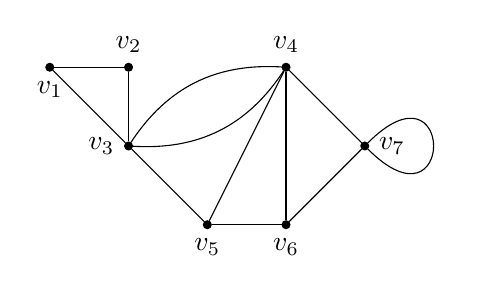
\begin{tikzpicture}
\tikzset{enclosed/.style={draw, circle, inner sep=0pt, minimum size=.10cm, fill=black}}
    \node[enclosed] at (1,2) (v_2) [label=above:\(v_2\)] {};
    \node[enclosed] at (3,2) (v_4) [label=above:\(v_4\)] {};
    \node[enclosed] at (4,1) (v_7) [label=right:\(v_7\)] {};
    \node[enclosed] at (2,0) (v_5) [label=below:\(v_5\)] {};
    \node[enclosed] at (3,0) (v_6) [label=below:\(v_6\)] {};
    \node[enclosed] at (1,1) (v_3) [label=left:\(v_3\)] {};
    \node[enclosed] at (0,2) (v_1) [label=below:\(v_1\)] {};

    \footnotesize
    \draw (v_2) -- (v_1);
    \path (v_3) edge [bend left] (v_4);
    \draw (v_2) -- (v_3);
    \path (v_3) edge [bend right] (v_4);
    \draw (v_4) -- (v_5);
    \draw (v_4) -- (v_6);
    \draw (v_4) -- (v_7);
    \draw (v_7) -- (v_6);
    \draw (v_7) to [out=315,in=45,looseness=50] (v_7);
    \draw (v_6) -- (v_5);
    \draw (v_5) -- (v_3);
    \draw (v_3) -- (v_1);
  \end{tikzpicture}
  \caption{Ikke-orienteret pseudograf.}
  \label{fig:ikke-orienteret-pseudo}
\end{figure}


\begin{table}[h]
\centering
\label{tab:naboliste-ikke-orienteret}
	\begin{tabular}{ |p{3cm}|p{3cm}|}
 		\hline
 		Knuder & Naboknuder\\
 		\hline
 		$v_1$ & $v_2$, $v_3$\\
		$v_2$ & $v_1$, $v_3$ \\
		$v_3$ & $v_1$, $v_2$, $v_4$, $v_5$ \\
		$v_4$ & $v_1$, $v_3$, $v_5$, $v_7$ \\
		$v_5$ & $v_3$, $v_4$, $v_6$ \\
		$v_6$ & $v_4$, $v_5$, $v_7$ \\
		$v_7$ & $v_4$, $v_6$, $v_7$ \\
 		\hline 
	\end{tabular}
	\caption{Naboliste til figur \ref{fig:ikke-orienteret-pseudo}}
\end{table}
